% ============================================================================
%  Persistent Homology for Parameter-Free Spectral Line Decomposition
%  AASTeX v6.3.1 — ApJ pre-print
% ============================================================================
\documentclass[twocolumn,twocolappendix]{aastex631}

% --- Packages ---------------------------------------------------------------
\usepackage{amsmath,amssymb}
\usepackage{graphicx}
\usepackage{tikz}
\usetikzlibrary{shapes.geometric,arrows.meta,positioning,calc,decorations.pathreplacing}
\usepackage{booktabs}
\usepackage{xcolor}

% --- Macros -----------------------------------------------------------------
\newcommand{\phspectra}{\textsc{phspectra}}
\newcommand{\gausspyp}{\textsc{GaussPy+}}
\newcommand{\gausspy}{\textsc{GaussPy}}
\newcommand{\rohsa}{\textsc{ROHSA}}
\newcommand{\spif}{\textsc{SPIF}}
\newcommand{\spectuner}{\textsc{Spectuner-D1}}
\newcommand{\srms}{\sigma_{\mathrm{rms}}}
\newcommand{\pmin}{\pi_{\mathrm{min}}}
\newcommand{\aicc}{\mathrm{AICc}}

% --- Metadata ---------------------------------------------------------------
\shorttitle{Persistent Homology for Spectral Line Decomposition}
\shortauthors{Vera-Ciro}

% ============================================================================
\begin{document}

\title{Persistent Homology for Parameter-Free Spectral Line Decomposition}

\author{Carlos Vera-Ciro}
\affiliation{Independent Researcher}

% ---------------------------------------------------------------------------
% ABSTRACT
% ---------------------------------------------------------------------------
\begin{abstract}
Decomposing radio spectral lines into individual Gaussian components is
essential for studying the interstellar medium, yet existing automated methods
require multiple trained parameters.  We present \phspectra, a new approach
that uses 0-dimensional persistent homology to detect peaks in 1D spectra.
Persistent homology tracks the birth and death of connected components in the
signal's upper-level sets as a threshold descends from the global maximum,
assigning each peak a topological persistence that measures its significance
without smoothing or differentiation.  The sole free parameter is $\beta$,
which sets the persistence threshold in units of noise:
$\pmin = \beta \cdot \srms$.  On a synthetic benchmark of 350 spectra spanning
seven difficulty categories, \phspectra\ achieves an overall F1 score of 0.916
at the default $\beta = 4.0$, with performance varying by less than 0.005
across $\beta \in [3.8, 4.5]$.  Compared with \gausspyp\ on 1000 real
${}^{13}$CO spectra from the Galactic Ring Survey, \phspectra\ produces lower
residual RMS in 68\% of head-to-head comparisons and runs 6.6$\times$ faster,
while requiring no parameter training.  The software is open-source and
available at \url{https://github.com/cavera/phspectra}.
\end{abstract}

\keywords{methods: data analysis --- ISM: kinematics and dynamics ---
          techniques: spectroscopic --- radio lines: ISM}

% ============================================================================
% §1  INTRODUCTION
% ============================================================================
\section{Introduction}\label{sec:intro}

% TODO: §1.1 — The spectral line decomposition problem
% - HI 21-cm, 13CO, other tracers as superpositions of Gaussians
% - Each component = one gas cloud along the line of sight
% - Blind decomposition: determine N_components + 3 params each (a, mu, sigma)
% - Scale of modern surveys: GALFA-HI (Peek+2018), THOR (Beuther+2016),
%   GRS (Jackson+2006) — millions of spectra

% TODO: §1.2 — Existing approaches
% - GaussPy (Lindner+2015): derivative spectroscopy, alpha_1, alpha_2 trained
% - GaussPy+ (Riener+2019): adds spatial coherence, still needs alpha training
% - ROHSA (Marchal+2019): regularized optimization, lambda weights
% - SPIF (Colombo+2024): GPU-accelerated fitting
% - Spectuner-D1 (Li+2025): deep reinforcement learning
% - Common limitation: multiple parameters requiring training or tuning

% TODO: §1.3 — This work
% - Persistent homology for peak detection — no prior application to spectral
%   decomposition in the literature
% - TDA in astronomy limited to cosmology: cosmic web topology (Xu+2019),
%   cosmic shear (Heydenreich+2022)
% - Single parameter beta, paper outline

% ============================================================================
% §2  METHOD
% ============================================================================
\section{Method}\label{sec:method}

We describe the \phspectra\ algorithm in four stages: peak detection via
persistent homology (\S\ref{sec:persistence}), conversion of topological peaks
to Gaussian candidates (\S\ref{sec:candidates}), nonlinear least-squares
fitting (\S\ref{sec:fitting}), and iterative refinement guided by the
corrected Akaike Information Criterion (\S\ref{sec:refinement}).

% ---------------------------------------------------------------------------
% §2.1  Persistent homology for 1D peak detection
% ---------------------------------------------------------------------------
\subsection{Persistent homology for 1D peak detection}\label{sec:persistence}

Given a discrete 1D signal $f : \{0, 1, \ldots, n{-}1\} \to \mathbb{R}$, we
define the \emph{upper-level set} at threshold $t$ as
\begin{equation}
  U_t = \bigl\{\, i \;\big|\; f(i) \geq t \,\bigr\}.
\end{equation}
As $t$ decreases from $\max(f)$ toward $-\infty$, the topology of $U_t$
changes: new connected components are \emph{born} when $t$ drops below a
local maximum, and two components \emph{merge} when their supporting
intervals connect.  At each merger, the younger component --- the one whose
maximum is lower --- \emph{dies} at the current threshold.  This is
0-dimensional persistent homology ($H_0$): tracking connected components
across a filtration parameterized by $t$
\citep{Edelsbrunner2002,Edelsbrunner2008}.

Each local maximum (except the global one) produces a birth--death pair
$(b, d)$ where $b = f(i)$ is the peak height, $d$ is the merge threshold,
and the \emph{persistence}
\begin{equation}\label{eq:persistence}
  \pi = b - d
\end{equation}
quantifies how prominent the peak is.  The global maximum never merges; it
has $d = 0$ and persistence equal to its height.  Persistence provides a
scale-independent ranking of peaks: high-persistence features correspond to
real signal; low-persistence features are noise fluctuations.  No smoothing
or differentiation is required.

\paragraph{Implementation.}
The algorithm processes samples in order of decreasing function value.  A
union-find data structure tracks connected components: when a newly visited
index has an already-visited neighbor belonging to a different component,
the two components are merged and the younger one's death is recorded.
Sorting the $n$ samples costs $O(n \log n)$; each union-find operation is
amortized $O(\alpha(n))$, where $\alpha$ is the inverse Ackermann function.
The total complexity is therefore $O(n \log n)$, dominated by the initial sort.

\paragraph{Persistence threshold.}
Raw persistence is measured in the same units as the signal, so a fixed
threshold cannot distinguish noise from signal across datasets with different
noise levels.  We set the minimum persistence in units of the noise:
\begin{equation}\label{eq:threshold}
  \pmin = \beta \cdot \srms,
\end{equation}
where $\srms$ is the noise RMS estimated from the data (see
\S\ref{sec:candidates}) and $\beta$ is the sole free parameter of the model.
The default value $\beta = 4.0$ corresponds to a $4\sigma$ persistence cut.

\paragraph{Visual intuition.}
Figure~\ref{fig:waterlevel} illustrates the descending-threshold process on a
synthetic three-peak spectrum.  As the threshold drops past each local
maximum, a new connected component (``island'') is born; when two islands
merge, the younger one dies and its persistence is recorded.  The three real
peaks have persistence values of $\pi = 2.58$, $1.20$, and $0.73$ ---
well separated from the near-zero persistence of noise fluctuations.

\begin{figure*}[t]
  \centering
  \includegraphics[width=\textwidth]{figures/img/water-level-stages.png}
  \caption{%
    The descending water-level interpretation of 0-dimensional persistent
    homology, applied to a synthetic three-peak spectrum.  As the threshold
    $t$ (dashed line) decreases, connected components are born at local maxima
    and die when they merge into an older component.  Red dots mark peak births;
    annotations show the final persistence $\pi = b - d$.  \emph{Top left}:
    $t$ above all peaks (empty upper-level set).  \emph{Top right}: peak~A
    ($\pi = 2.58$) is born as the global maximum.  \emph{Bottom left}: peak~B
    ($\pi = 1.20$) appears as a second island.  \emph{Bottom right}: peak~C
    ($\pi = 0.73$) dies when its island merges with~A's.
    \label{fig:waterlevel}}
\end{figure*}

Figure~\ref{fig:persistence_diagram} shows the corresponding persistence
diagram.  Each peak is plotted as a point $(b, d)$ in birth--death space; the
diagonal $b = d$ represents zero persistence.  The three real peaks (red)
are clearly separated from the cluster of noise points (grey) near the
diagonal, illustrating that any persistence threshold drawn through this gap
cleanly separates signal from noise.

\begin{figure}[t]
  \centering
  \includegraphics[width=\columnwidth]{figures/img/persistence-diagram.png}
  \caption{%
    Persistence diagram for the synthetic spectrum in
    Figure~\ref{fig:waterlevel}.  Each local maximum is plotted at its
    birth--death coordinates $(b, d)$.  The three real peaks (red) sit well
    above the diagonal, while noise fluctuations (grey) cluster near
    $b \approx d$.  The horizontal dashed line indicates the persistence
    threshold $\pmin = \beta \cdot \srms$.
    \label{fig:persistence_diagram}}
\end{figure}

% ---------------------------------------------------------------------------
% §2.2  From persistence to Gaussian candidates
% ---------------------------------------------------------------------------
\subsection{From persistence to Gaussian candidates}\label{sec:candidates}

\paragraph{Noise estimation.}
Before peak detection, \phspectra\ estimates $\srms$ using a signal-masked
approach following \citet{Riener2019}, Section~3.1.1.  Runs of more than two
consecutive positive channels are masked (with two-channel padding on each
side) to exclude spectral features.  The median absolute deviation (MAD) of
the remaining negative channels provides an initial robust scale estimate.
Channels exceeding $\pm 5\,\sigma_{\mathrm{MAD}}$ are then clipped, and the
final RMS is computed as $\srms = \sqrt{\langle x^2 \rangle}$ over the
surviving channels.  This procedure avoids biasing the noise estimate with
real emission.

\paragraph{Initial Gaussian guesses.}
Each peak surviving the persistence threshold $\pmin = \beta \cdot \srms$ is
converted to an initial Gaussian guess with three parameters:
\begin{itemize}
  \item \emph{Amplitude}: the signal value at the peak's channel index,
        $a_0 = f(\mathrm{index})$.
  \item \emph{Mean}: the peak's channel index.
  \item \emph{Standard deviation}: a fixed initial value $\sigma_0 = 1.0$
        channel.  The persistence filtration determines \emph{where} peaks are
        and \emph{how significant} they are, but provides no width information;
        the width is recovered entirely by the subsequent least-squares fit.
\end{itemize}
Peaks are ordered by persistence (most significant first), so when a
\texttt{max\_components} cap is set, the least significant surviving peaks
are dropped.

% ---------------------------------------------------------------------------
% §2.3  Gaussian fitting
% ---------------------------------------------------------------------------
\subsection{Gaussian fitting}\label{sec:fitting}

The initial guesses are fitted simultaneously as a sum of $K$ Gaussians:
\begin{equation}\label{eq:model}
  F(x) = \sum_{i=1}^{K} a_i \exp\!\left(-\frac{(x - \mu_i)^2}{2\sigma_i^2}\right),
\end{equation}
using bounded nonlinear least-squares optimization via
\texttt{scipy.optimize.curve\_fit} \citep{Virtanen2020}.  The bounds enforce
$a_i \geq 0$, $\mu_i \in [0, n)$, and $\sigma_i \in [0.3, n/2]$ channels.
Because the persistence-detected peak positions and amplitudes are already
close to the true values, the optimizer typically converges in few iterations
--- its primary task is to determine the correct widths and fine-tune
positions and amplitudes.

% ---------------------------------------------------------------------------
% §2.4  Iterative refinement
% ---------------------------------------------------------------------------
\subsection{Iterative refinement}\label{sec:refinement}

When refinement is enabled (the default), the initial fit is iteratively
improved through a loop of up to three iterations.  Each modification is
accepted only if it decreases the corrected Akaike Information Criterion
\citep{Akaike1974,Hurvich1989}:
\begin{equation}\label{eq:aicc}
  \aicc = N \ln\!\left(\frac{\mathrm{RSS}}{N}\right) + 2k
        + \frac{2k^2 + 2k}{N - k - 1},
\end{equation}
where $\mathrm{RSS} = \sum_j (f_j - F_j)^2$ is the residual sum of squares,
$k = 3K$ is the number of free parameters (three per Gaussian component),
and $N$ is the number of spectral channels.

Each refinement iteration performs four operations:

\begin{enumerate}
  \item \textbf{Component validation.}  Components are rejected if any of the
    following hold: (a)~FWHM $< 1$ channel; (b)~mean outside the spectrum;
    (c)~amplitude $< 1.5\,\srms$ (SNR floor); or (d)~significance $< 4.0$,
    where the significance of component~$i$ is defined as
    \begin{equation}\label{eq:significance}
      S_i = \frac{W_i}{\sqrt{2\,\mathrm{FWHM}_i}\;\srms},
    \end{equation}
    with integrated flux
    $W_i = a_i \, \sigma_i \, \sqrt{2\pi}$.

  \item \textbf{Residual peak search.}  The persistence detection algorithm is
    run on the residual spectrum (data minus model) with a lower threshold of
    $1.5\,\srms$ to find missed components.  Any peaks found are added to the
    model and validated.

  \item \textbf{Negative dip splitting.}  If the residual contains a dip
    exceeding $-5\,\srms$, the broadest Gaussian component overlapping that
    channel is split into two narrower components.

  \item \textbf{Blended pair merging.}  If two components are separated by
    less than $1.2 \times \min(\mathrm{FWHM}_i, \mathrm{FWHM}_j)$, they are
    merged into a single flux-weighted component.
\end{enumerate}

After each operation, the full model is refit via least-squares, and the
modification is accepted only if $\aicc$ decreases.  The loop terminates when
no operation produces an improvement or the iteration limit is reached.

Figure~\ref{fig:pipeline} summarizes the complete pipeline from raw spectrum
to final Gaussian components.

\begin{figure}[t]
  \centering
  \resizebox{\columnwidth}{!}{% Pipeline overview flowchart for phspectra
% Included via % Pipeline overview flowchart for phspectra
% Included via % Pipeline overview flowchart for phspectra
% Included via \input{figures/tikz/pipeline-overview.tex} in ms.tex
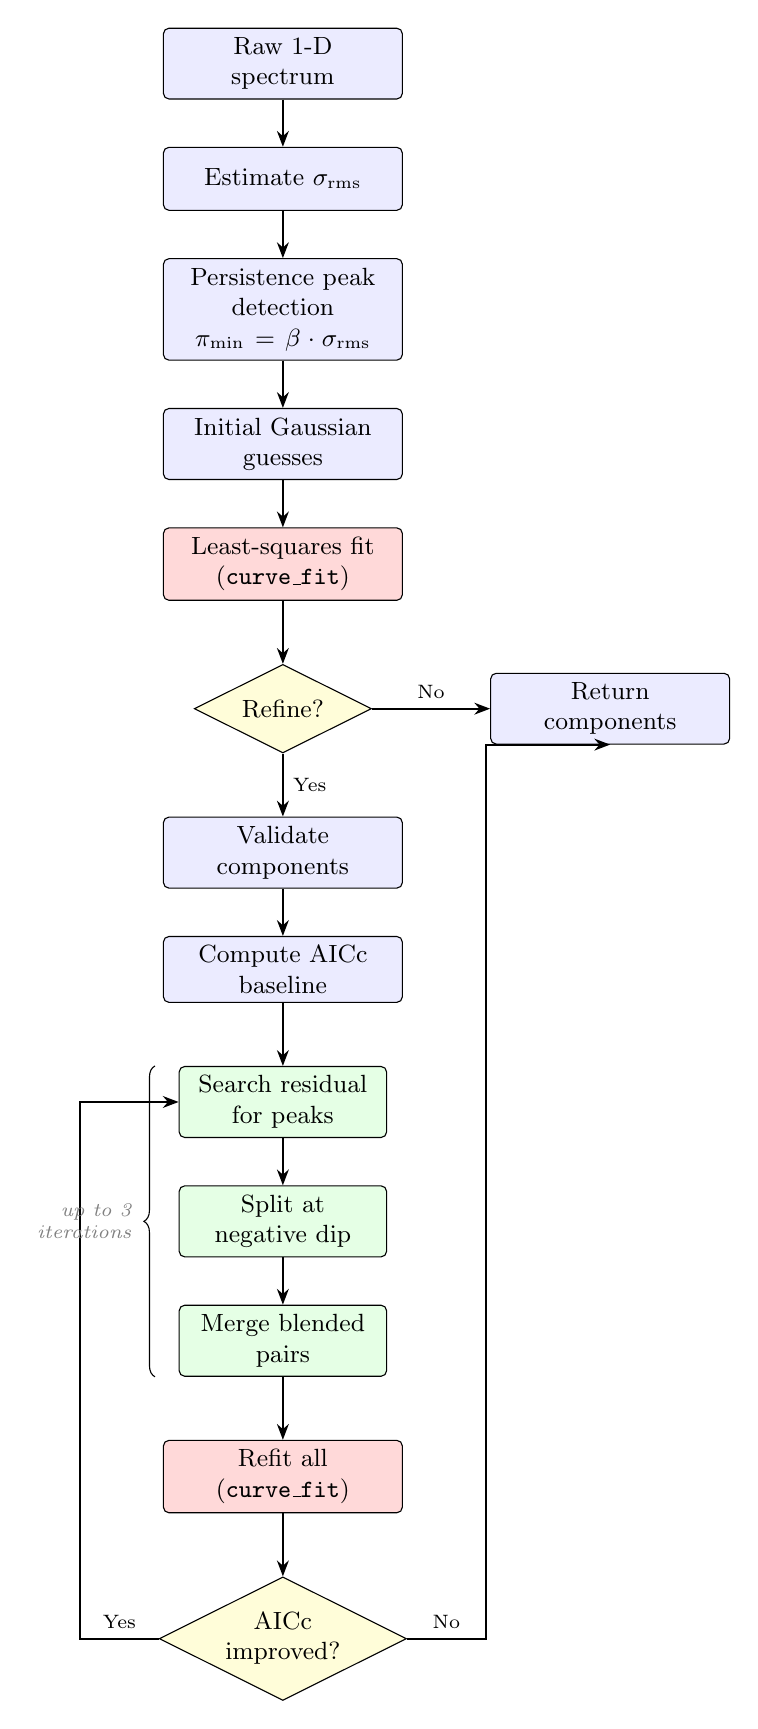
\begin{tikzpicture}[
    node distance=6mm and 4mm,
    every node/.style={font=\small},
    block/.style={
      rectangle, draw, rounded corners=2pt,
      text width=28mm, minimum height=8mm,
      align=center, fill=blue!8
    },
    decision/.style={
      diamond, draw, aspect=2,
      text width=16mm, align=center,
      inner sep=1pt, fill=yellow!15
    },
    fitblock/.style={
      rectangle, draw, rounded corners=2pt,
      text width=28mm, minimum height=8mm,
      align=center, fill=red!15
    },
    refineblock/.style={
      rectangle, draw, rounded corners=2pt,
      text width=24mm, minimum height=7mm,
      align=center, fill=green!10
    },
    arr/.style={-{Stealth[length=2mm]}, thick},
    note/.style={font=\scriptsize\itshape, text=gray}
  ]

  % Main pipeline
  \node[block] (input) {Raw 1-D\\spectrum};
  \node[block, below=of input] (rms) {Estimate $\srms$};
  \node[block, below=of rms] (persist) {Persistence peak\\detection\\$\pmin = \beta \cdot \srms$};
  \node[block, below=of persist] (guess) {Initial Gaussian\\guesses};
  \node[fitblock, below=of guess] (fit) {Least-squares fit\\(\texttt{curve\_fit})};
  \node[decision, below=8mm of fit] (refineq) {Refine?};

  % No-refine path
  \node[block, right=15mm of refineq] (output) {Return\\components};

  % Refine path
  \node[block, below=8mm of refineq] (validate) {Validate\\components};
  \node[block, below=of validate] (aiccbase) {Compute AICc\\baseline};

  % Refinement loop
  \node[refineblock, below=8mm of aiccbase] (residual) {Search residual\\for peaks};
  \node[refineblock, below=of residual] (split) {Split at\\negative dip};
  \node[refineblock, below=of split] (merge) {Merge blended\\pairs};
  \node[fitblock, below=8mm of merge] (refit) {Refit all\\(\texttt{curve\_fit})};
  \node[decision, below=8mm of refit] (improved) {AICc\\improved?};

  % Arrows — main path
  \draw[arr] (input) -- (rms);
  \draw[arr] (rms) -- (persist);
  \draw[arr] (persist) -- (guess);
  \draw[arr] (guess) -- (fit);
  \draw[arr] (fit) -- (refineq);
  \draw[arr] (refineq) -- node[above] {\scriptsize No} (output);
  \draw[arr] (refineq) -- node[right] {\scriptsize Yes} (validate);
  \draw[arr] (validate) -- (aiccbase);
  \draw[arr] (aiccbase) -- (residual);
  \draw[arr] (residual) -- (split);
  \draw[arr] (split) -- (merge);
  \draw[arr] (merge) -- (refit);
  \draw[arr] (refit) -- (improved);

  % Accept → loop back
  \draw[arr] (improved.west) -- ++(-10mm,0)
    node[above, pos=0.5] {\scriptsize Yes}
    |- (residual.west);

  % Reject → output
  \draw[arr] (improved.east) -- ++(10mm,0)
    node[above, pos=0.5] {\scriptsize No}
    |- (output.south);

  % Brace for refinement loop
  \draw[decorate, decoration={brace, amplitude=4pt, mirror}]
    ([xshift=-3mm]residual.north west) -- ([xshift=-3mm]merge.south west)
    node[midway, left=5pt, note, text width=12mm, align=right]
    {up to 3\\iterations};

\end{tikzpicture}
 in ms.tex
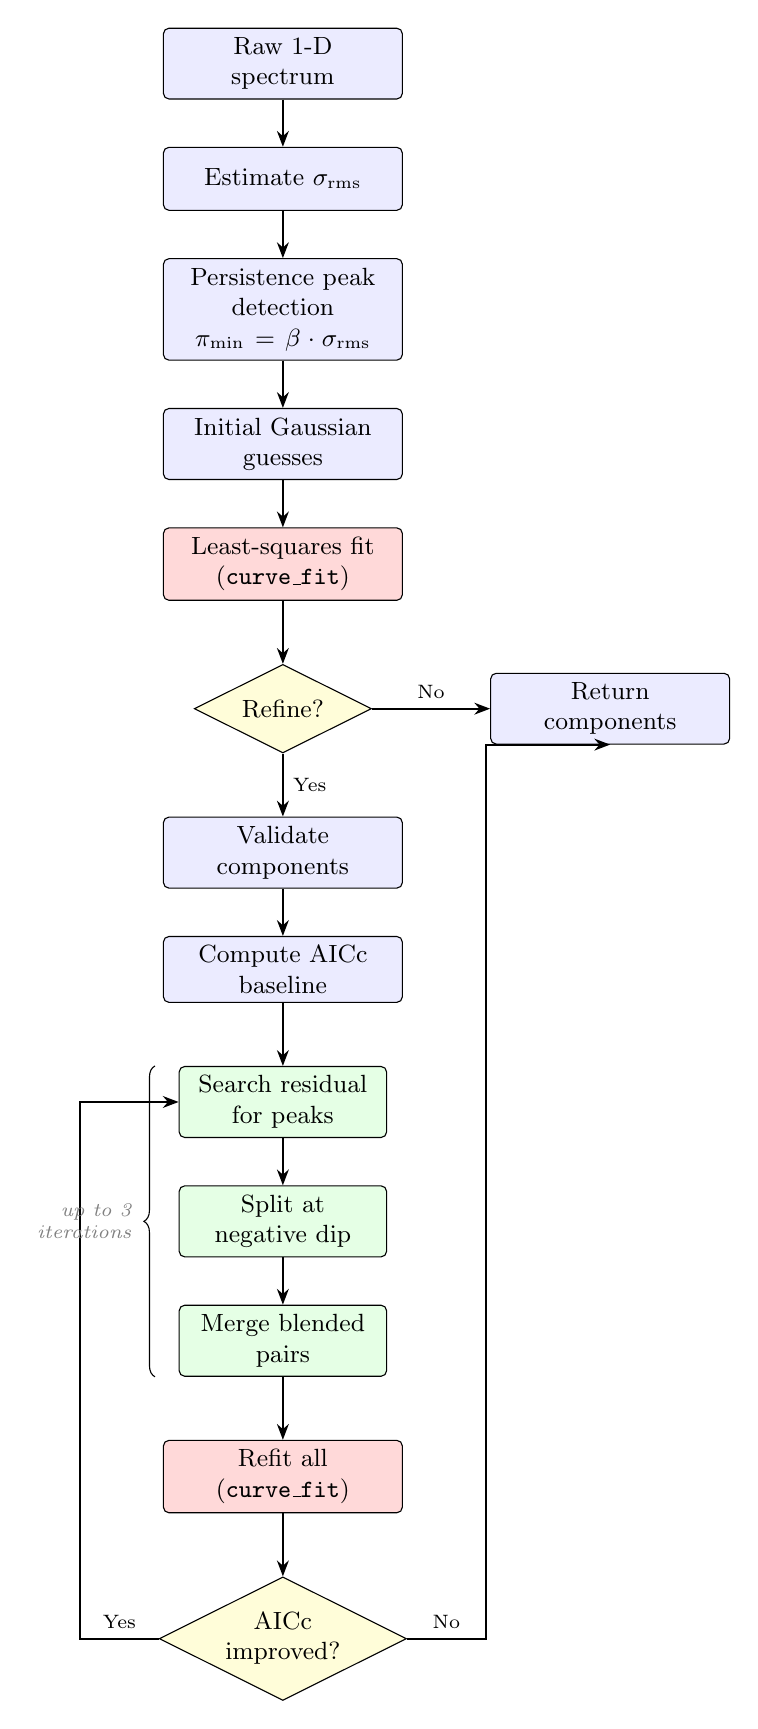
\begin{tikzpicture}[
    node distance=6mm and 4mm,
    every node/.style={font=\small},
    block/.style={
      rectangle, draw, rounded corners=2pt,
      text width=28mm, minimum height=8mm,
      align=center, fill=blue!8
    },
    decision/.style={
      diamond, draw, aspect=2,
      text width=16mm, align=center,
      inner sep=1pt, fill=yellow!15
    },
    fitblock/.style={
      rectangle, draw, rounded corners=2pt,
      text width=28mm, minimum height=8mm,
      align=center, fill=red!15
    },
    refineblock/.style={
      rectangle, draw, rounded corners=2pt,
      text width=24mm, minimum height=7mm,
      align=center, fill=green!10
    },
    arr/.style={-{Stealth[length=2mm]}, thick},
    note/.style={font=\scriptsize\itshape, text=gray}
  ]

  % Main pipeline
  \node[block] (input) {Raw 1-D\\spectrum};
  \node[block, below=of input] (rms) {Estimate $\srms$};
  \node[block, below=of rms] (persist) {Persistence peak\\detection\\$\pmin = \beta \cdot \srms$};
  \node[block, below=of persist] (guess) {Initial Gaussian\\guesses};
  \node[fitblock, below=of guess] (fit) {Least-squares fit\\(\texttt{curve\_fit})};
  \node[decision, below=8mm of fit] (refineq) {Refine?};

  % No-refine path
  \node[block, right=15mm of refineq] (output) {Return\\components};

  % Refine path
  \node[block, below=8mm of refineq] (validate) {Validate\\components};
  \node[block, below=of validate] (aiccbase) {Compute AICc\\baseline};

  % Refinement loop
  \node[refineblock, below=8mm of aiccbase] (residual) {Search residual\\for peaks};
  \node[refineblock, below=of residual] (split) {Split at\\negative dip};
  \node[refineblock, below=of split] (merge) {Merge blended\\pairs};
  \node[fitblock, below=8mm of merge] (refit) {Refit all\\(\texttt{curve\_fit})};
  \node[decision, below=8mm of refit] (improved) {AICc\\improved?};

  % Arrows — main path
  \draw[arr] (input) -- (rms);
  \draw[arr] (rms) -- (persist);
  \draw[arr] (persist) -- (guess);
  \draw[arr] (guess) -- (fit);
  \draw[arr] (fit) -- (refineq);
  \draw[arr] (refineq) -- node[above] {\scriptsize No} (output);
  \draw[arr] (refineq) -- node[right] {\scriptsize Yes} (validate);
  \draw[arr] (validate) -- (aiccbase);
  \draw[arr] (aiccbase) -- (residual);
  \draw[arr] (residual) -- (split);
  \draw[arr] (split) -- (merge);
  \draw[arr] (merge) -- (refit);
  \draw[arr] (refit) -- (improved);

  % Accept → loop back
  \draw[arr] (improved.west) -- ++(-10mm,0)
    node[above, pos=0.5] {\scriptsize Yes}
    |- (residual.west);

  % Reject → output
  \draw[arr] (improved.east) -- ++(10mm,0)
    node[above, pos=0.5] {\scriptsize No}
    |- (output.south);

  % Brace for refinement loop
  \draw[decorate, decoration={brace, amplitude=4pt, mirror}]
    ([xshift=-3mm]residual.north west) -- ([xshift=-3mm]merge.south west)
    node[midway, left=5pt, note, text width=12mm, align=right]
    {up to 3\\iterations};

\end{tikzpicture}
 in ms.tex
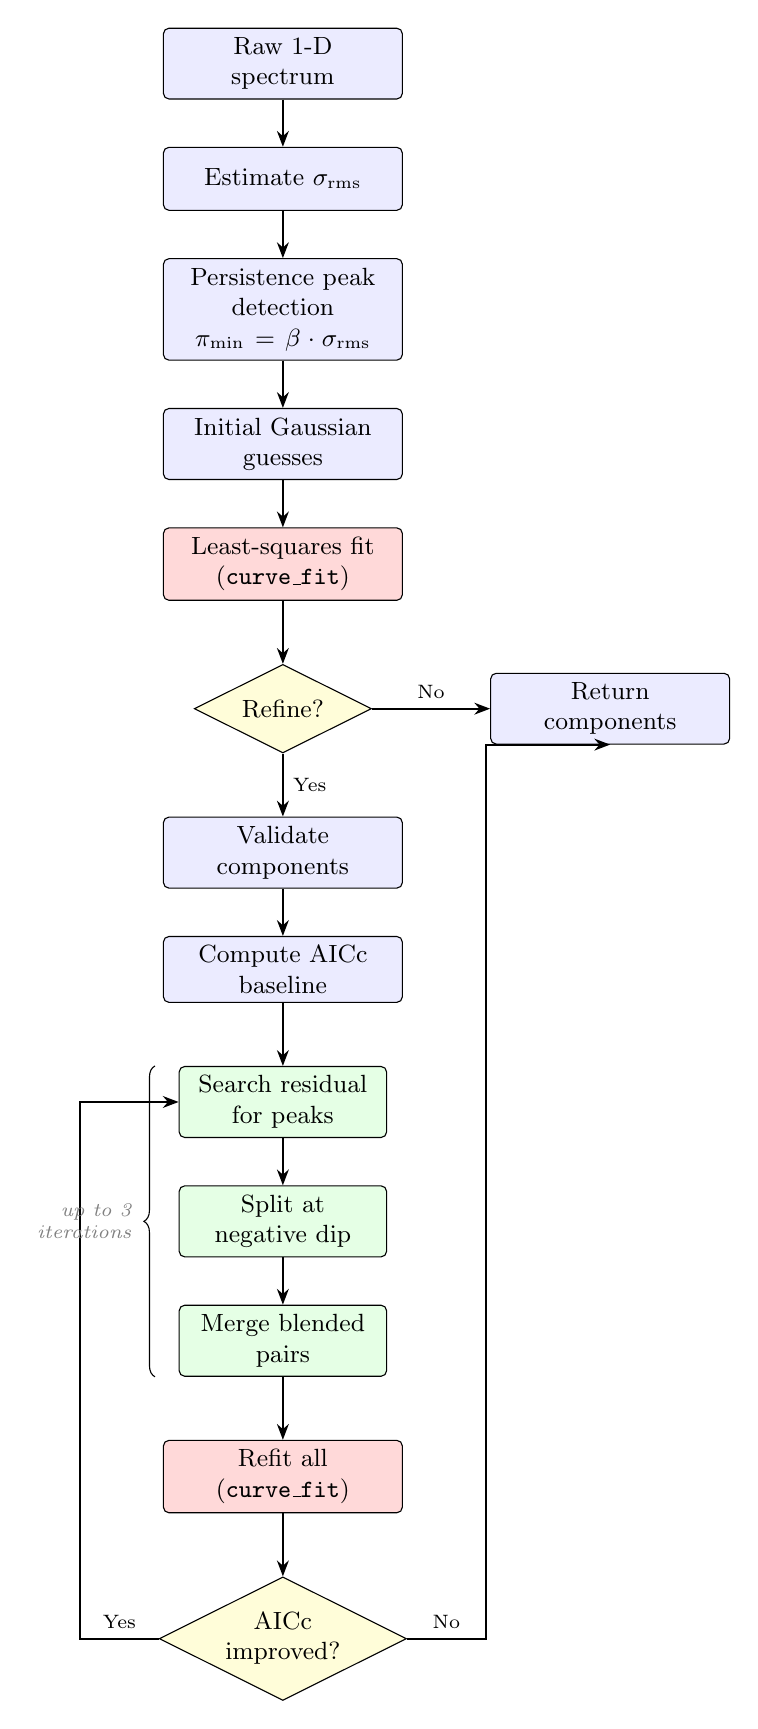
\begin{tikzpicture}[
    node distance=6mm and 4mm,
    every node/.style={font=\small},
    block/.style={
      rectangle, draw, rounded corners=2pt,
      text width=28mm, minimum height=8mm,
      align=center, fill=blue!8
    },
    decision/.style={
      diamond, draw, aspect=2,
      text width=16mm, align=center,
      inner sep=1pt, fill=yellow!15
    },
    fitblock/.style={
      rectangle, draw, rounded corners=2pt,
      text width=28mm, minimum height=8mm,
      align=center, fill=red!15
    },
    refineblock/.style={
      rectangle, draw, rounded corners=2pt,
      text width=24mm, minimum height=7mm,
      align=center, fill=green!10
    },
    arr/.style={-{Stealth[length=2mm]}, thick},
    note/.style={font=\scriptsize\itshape, text=gray}
  ]

  % Main pipeline
  \node[block] (input) {Raw 1-D\\spectrum};
  \node[block, below=of input] (rms) {Estimate $\srms$};
  \node[block, below=of rms] (persist) {Persistence peak\\detection\\$\pmin = \beta \cdot \srms$};
  \node[block, below=of persist] (guess) {Initial Gaussian\\guesses};
  \node[fitblock, below=of guess] (fit) {Least-squares fit\\(\texttt{curve\_fit})};
  \node[decision, below=8mm of fit] (refineq) {Refine?};

  % No-refine path
  \node[block, right=15mm of refineq] (output) {Return\\components};

  % Refine path
  \node[block, below=8mm of refineq] (validate) {Validate\\components};
  \node[block, below=of validate] (aiccbase) {Compute AICc\\baseline};

  % Refinement loop
  \node[refineblock, below=8mm of aiccbase] (residual) {Search residual\\for peaks};
  \node[refineblock, below=of residual] (split) {Split at\\negative dip};
  \node[refineblock, below=of split] (merge) {Merge blended\\pairs};
  \node[fitblock, below=8mm of merge] (refit) {Refit all\\(\texttt{curve\_fit})};
  \node[decision, below=8mm of refit] (improved) {AICc\\improved?};

  % Arrows — main path
  \draw[arr] (input) -- (rms);
  \draw[arr] (rms) -- (persist);
  \draw[arr] (persist) -- (guess);
  \draw[arr] (guess) -- (fit);
  \draw[arr] (fit) -- (refineq);
  \draw[arr] (refineq) -- node[above] {\scriptsize No} (output);
  \draw[arr] (refineq) -- node[right] {\scriptsize Yes} (validate);
  \draw[arr] (validate) -- (aiccbase);
  \draw[arr] (aiccbase) -- (residual);
  \draw[arr] (residual) -- (split);
  \draw[arr] (split) -- (merge);
  \draw[arr] (merge) -- (refit);
  \draw[arr] (refit) -- (improved);

  % Accept → loop back
  \draw[arr] (improved.west) -- ++(-10mm,0)
    node[above, pos=0.5] {\scriptsize Yes}
    |- (residual.west);

  % Reject → output
  \draw[arr] (improved.east) -- ++(10mm,0)
    node[above, pos=0.5] {\scriptsize No}
    |- (output.south);

  % Brace for refinement loop
  \draw[decorate, decoration={brace, amplitude=4pt, mirror}]
    ([xshift=-3mm]residual.north west) -- ([xshift=-3mm]merge.south west)
    node[midway, left=5pt, note, text width=12mm, align=right]
    {up to 3\\iterations};

\end{tikzpicture}
}
  \caption{%
    Flowchart of the \phspectra\ pipeline.  The algorithm proceeds from noise
    estimation through persistence-based peak detection, initial Gaussian
    fitting, and iterative refinement.  Each refinement step (residual search,
    dip splitting, blended merging) is accepted only if it lowers the AICc.
    \label{fig:pipeline}}
\end{figure}


% ============================================================================
% §3  EVALUATION
% ============================================================================
\section{Evaluation}\label{sec:evaluation}

We evaluate \phspectra\ on both synthetic spectra with known ground-truth
components (\S\ref{sec:synthetic}) and real ${}^{13}$CO data from the Galactic
Ring Survey (\S\ref{sec:grs}).

% ---------------------------------------------------------------------------
% §3.1  Synthetic benchmark
% ---------------------------------------------------------------------------
\subsection{Synthetic benchmark}\label{sec:synthetic}

\paragraph{Test design.}
We construct a benchmark of 350 synthetic spectra ($50$ per category) spanning
seven categories of increasing difficulty (Table~\ref{tab:categories}).  Each
spectrum has 424 channels with additive Gaussian noise at $\sigma = 0.13$~K,
matching the properties of the GRS \citep{Jackson2006}.  Because the true
Gaussian components are known exactly, the F1 score measures true accuracy
rather than agreement with another algorithm.

Component matching uses the Hungarian algorithm with the criteria of
\citet{Lindner2015}: a predicted component matches a true component if the
amplitude ratio is within $[0.5, 2.0]$, the position difference is less than
the larger of the two widths, and the width ratio is within $[0.5, 2.0]$.
F1 is computed as the harmonic mean of precision (fraction of predicted
components that match a true one) and recall (fraction of true components that
are matched).

\begin{deluxetable}{llcccl}
\tablecaption{Synthetic benchmark categories.  Each category contains 50
spectra with the listed parameter ranges and constraints.  All spectra have
424 channels and noise $\sigma = 0.13$~K.\label{tab:categories}}
\tablehead{
  \colhead{Category} & \colhead{Label} & \colhead{$N_{\mathrm{comp}}$} &
  \colhead{$a$ (K)} & \colhead{$\sigma$ (ch)} & \colhead{Constraint}
}
\startdata
Single Bright    & SB  & 1   & 1.0--5.0  & 3--10  & SNR $> 7$         \\
Single Faint     & SF  & 1   & 0.3--0.8  & 3--10  & SNR $2$--$6$      \\
Single Narrow    & SN  & 1   & 1.0--5.0  & 1--2.5 & Sub-resolution    \\
Single Broad     & SBd & 1   & 0.5--3.0  & 10--20 & Extended features \\
Multi Separated  & MS  & 2--3 & 0.5--4.0 & 2--8   & Sep.\ $> 4\sigma$ \\
Multi Blended    & MB  & 2--3 & 0.5--4.0 & 3--8   & Sep.\ $1.5$--$3\sigma$ \\
Crowded          & C   & 4--5 & 0.3--3.0 & 2--6   & Mixed separations \\
\enddata
\end{deluxetable}

\paragraph{Results.}
Figure~\ref{fig:synthetic_f1} shows the F1 score as a function of $\beta$ for
each category and overall.  The overall F1 varies by only 0.005 across the
full sweep from $\beta = 3.8$ to $\beta = 4.5$, confirming the negligible
sensitivity of the algorithm to this parameter.  At the optimal
$\beta = 3.8$, the overall F1 is 0.916.

The difficulty gradient follows physical expectations:
well-separated multi-component spectra (MS) are easiest (F1~$= 0.965$), while
heavily blended multi-component spectra (MB) are the most challenging
(F1~$= 0.849$), a regime where any algorithm faces fundamental ambiguity due
to overlapping components.  Table~\ref{tab:f1} lists the per-category F1
scores.

\begin{figure}[t]
  \centering
  \includegraphics[width=\columnwidth]{figures/img/synthetic-f1.png}
  \caption{%
    F1 score versus $\beta$ for each synthetic benchmark category (colored
    lines) and overall (black).  Performance is remarkably stable: the overall
    F1 varies by only 0.005 across $\beta \in [3.8, 4.5]$.
    \label{fig:synthetic_f1}}
\end{figure}

\begin{deluxetable}{llc}
\tablecaption{Per-category F1 scores on the synthetic benchmark at the
optimal $\beta$.\label{tab:f1}}
\tablehead{
  \colhead{Category} & \colhead{Label} & \colhead{F1}
}
\startdata
Multi Separated  & MS  & 0.965 \\
Single Broad     & SBd & 0.935 \\
Crowded          & C   & 0.933 \\
Single Bright    & SB  & 0.926 \\
Single Narrow    & SN  & 0.909 \\
Single Faint     & SF  & 0.863 \\
Multi Blended    & MB  & 0.849 \\
\enddata
\end{deluxetable}

\paragraph{Parameter recovery.}
Figure~\ref{fig:synthetic_errors} shows the amplitude relative error, position
error (in channels), and width relative error across the $\beta$ sweep.
Position errors are sub-channel for most categories; amplitude and width
relative errors are small and stable across the tested range.

\begin{figure}[t]
  \centering
  \includegraphics[width=\columnwidth]{figures/img/synthetic-errors.png}
  \caption{%
    Parameter recovery on the synthetic benchmark.  Box-whisker plots show the
    amplitude relative error, position error (channels), and width relative
    error for matched components across $\beta \in [3.8, 4.5]$.  Errors are
    small and stable across the full range.
    \label{fig:synthetic_errors}}
\end{figure}

% ---------------------------------------------------------------------------
% §3.2  GRS comparison with GaussPy+
% ---------------------------------------------------------------------------
\subsection{GRS comparison with GaussPy+}\label{sec:grs}

We compare \phspectra\ and \gausspyp\ on 1000 randomly selected spectra from
the Galactic Ring Survey \citep[GRS;][]{Jackson2006}, a ${}^{13}$CO $J = 1
\to 0$ survey of the inner Galaxy.  Each spectrum has 424 velocity channels.
\gausspyp\ is run in its Docker container using the \texttt{GaussPyDecompose}
module with the trained parameters from \citet{Riener2019}: $\alpha_1 = 2.89$,
$\alpha_2 = 6.65$ (two-phase decomposition), and an SNR threshold of 3.0.
\phspectra\ uses the default $\beta = 4.0$.

\subsubsection{Residual RMS}\label{sec:rms}

Table~\ref{tab:rms} summarizes the fit quality.  Both tools fit most spectra
near the noise floor ($\sigma = 0.13$~K), with nearly identical mean RMS
values.  However, in head-to-head comparisons, \phspectra\ achieves lower
residual RMS on 68\% of spectra (683 of 1000).  The slightly lower mean RMS
of \gausspyp\ is driven by a tail of spectra where it fits many more
components, reducing RMS at the cost of potential overfitting.

\begin{deluxetable}{lcc}
\tablecaption{Residual RMS comparison on 1000 GRS spectra.\label{tab:rms}}
\tablehead{
  \colhead{Metric} & \colhead{\phspectra} & \colhead{\gausspyp}
}
\startdata
Mean RMS (K)     & 0.1303 & 0.1300 \\
Lower RMS wins   & \textbf{683} (68\%) & 317 (32\%) \\
\enddata
\end{deluxetable}

Figure~\ref{fig:rms_dist} shows the RMS distributions for both tools; the
distributions overlap heavily, confirming comparable overall fit quality.
Figure~\ref{fig:rms_scatter} shows a scatter plot of per-spectrum RMS values;
the majority of points fall below the 1:1 line, indicating lower \phspectra\
residuals.

\begin{figure}[t]
  \centering
  \includegraphics[width=\columnwidth]{figures/img/rms-distribution.png}
  \caption{%
    Distribution of per-spectrum residual RMS for \phspectra\ (blue) and
    \gausspyp\ (orange) on 1000 GRS spectra.  Both distributions peak near the
    noise floor ($\sigma = 0.13$~K).
    \label{fig:rms_dist}}
\end{figure}

\begin{figure}[t]
  \centering
  \includegraphics[width=\columnwidth]{figures/img/rms-scatter.png}
  \caption{%
    Per-spectrum residual RMS: \phspectra\ versus \gausspyp.  Points below the
    1:1 line (dashed) indicate spectra where \phspectra\ achieves lower
    residual RMS.
    \label{fig:rms_scatter}}
\end{figure}

\subsubsection{Decomposition disagreements}\label{sec:disagreements}

A systematic comparison reveals several recurring patterns of disagreement
between the two tools (Figure~\ref{fig:disagreements}).  \gausspyp\ sometimes
fits many components (up to 14) where \phspectra\ finds fewer,
better-constrained ones; conversely, \phspectra\ can resolve blended features
that \gausspyp\ misses.  Even when both tools detect the same number of
components, they may place them at different positions or assign different
widths.  These patterns are not systematic failures of either tool --- they
reflect genuinely different decomposition strategies applied to the same
ambiguous data.

\begin{figure*}[t]
  \centering
  \includegraphics[width=\textwidth]{figures/img/compare-disagreements.png}
  \caption{%
    Representative disagreement cases between \phspectra\ and \gausspyp\ on
    GRS spectra.  Each panel shows the data (black), \phspectra\ fit (blue),
    and \gausspyp\ fit (orange).  Cases include: \phspectra\ finding fewer
    components, \phspectra\ resolving blended features, each tool achieving
    lower RMS on different spectra, and decompositions with the same component
    count but different positions or widths.
    \label{fig:disagreements}}
\end{figure*}

\subsubsection{Component widths}\label{sec:widths}

A population-level comparison of fitted widths shows no systematic bias
between the two tools.  Matching 644 component pairs across 1000 spectra
using the Hungarian algorithm with a position tolerance of $2\sigma$, the
median log-width ratio $\ln(\sigma_{\mathrm{ph}} / \sigma_{\mathrm{GP+}})$
is near zero, and the split is near even: \gausspyp\ fits wider profiles
in 55\% of pairs, \phspectra\ in 45\%.

Figure~\ref{fig:widths} shows the histogram of log-width ratios, which is
sharply peaked at zero.  Individual spectra can show large width differences
(as in Figure~\ref{fig:disagreements}), but these are isolated instances
driven by different decomposition strategies, not a systematic effect.

\begin{figure}[t]
  \centering
  \includegraphics[width=\columnwidth]{figures/img/width-comparison.png}
  \caption{%
    Distribution of log-width ratios
    $\ln(\sigma_{\mathrm{ph}} / \sigma_{\mathrm{GP+}})$ for 644 matched
    component pairs.  The distribution is sharply peaked at zero, indicating
    no systematic width bias between the two tools.
    \label{fig:widths}}
\end{figure}


% ============================================================================
% §4  PARAMETER SENSITIVITY
% ============================================================================
\section{Parameter sensitivity}\label{sec:beta}

% TODO: Full prose for this section.  Key points:
% - beta sweep on real GRS data (200 spectra): F1 varies by only ~0.01
%   across beta in [3.8, 4.5], optimal beta = 4.0 with F1 = 0.847
% - The F1 ceiling reflects disagreement between algorithms, not a
%   limitation of phspectra (see §3.2)
% - Comparison with GaussPy alpha training requirements:
%   alpha must be trained per survey/region on synthetic spectra;
%   beta requires no training — default works across surveys
% - Physically interpretable: beta = 4.0 means "reject peaks with
%   persistence < 4 sigma" — a natural significance threshold
% - Recommendation: beta = 4.0 for general use

\begin{figure}[t]
  \centering
  \includegraphics[width=\columnwidth]{figures/img/f1-beta-sweep.png}
  \caption{%
    F1 score versus $\beta$ on 200 real GRS spectra, scored against
    \gausspyp\ catalog decompositions \citep{Riener2020}.  The curve is nearly
    flat across $\beta \in [3.8, 4.5]$, with $\Delta\mathrm{F1} \approx 0.01$.
    The optimal $\beta = 4.0$ achieves F1~$= 0.847$.
    \label{fig:beta_sweep}}
\end{figure}


% ============================================================================
% §5  PERFORMANCE
% ============================================================================
\section{Performance}\label{sec:performance}

% TODO: Full prose for this section.  Key points:
% - Benchmark: 1000 GRS spectra (424 channels each), single-core
% - phspectra: beta = 4.0, native Python 3.14
% - GaussPy+: Docker, Python 3.10, trained alpha values
% - Results: phspectra 123.5s vs GaussPy+ 812.5s → 6.6× faster
% - Mean per spectrum: 124ms vs 813ms
% - Mean components detected: 2.7 vs 2.4
% - Why faster: (1) no smoothing sweep, (2) fewer optimization steps,
%   (3) no training overhead

\begin{deluxetable}{lccc}
\tablecaption{Wall-clock timing benchmark on 1000 GRS spectra.
\label{tab:timing}}
\tablehead{
  \colhead{Metric} & \colhead{\phspectra} & \colhead{\gausspyp} &
  \colhead{Factor}
}
\startdata
Total time        & 123.5\,s & 812.5\,s & $6.6\times$ \\
Per spectrum      & 124\,ms  & 813\,ms  & $6.6\times$ \\
Components found  & 2.7      & 2.4      & ---         \\
\enddata
\end{deluxetable}

\begin{figure}[t]
  \centering
  \includegraphics[width=\columnwidth]{figures/img/performance-benchmark.png}
  \caption{%
    Per-spectrum decomposition time for \phspectra\ (blue) and \gausspyp\
    (orange) on 1000 GRS spectra.  \phspectra\ is $6.6\times$ faster on
    average.
    \label{fig:performance}}
\end{figure}


% ============================================================================
% §6  DISCUSSION
% ============================================================================
\section{Discussion}\label{sec:discussion}

% TODO: Full prose for this section.  Key points:
% - Scalability: serverless pipeline exists (AWS Lambda), millions of spectra
%   feasible; beyond the scope of this paper
% - Limitations:
%   (1) No spatial coherence — each spectrum decomposed independently;
%       GaussPy+ enforces coherence across neighboring pixels (Riener+2019
%       Sect 3.3).  Future extension.
%   (2) Single beta for all spectra — could vary across survey regions,
%       though §4 shows this is not critical
%   (3) Assumes Gaussian line profiles — non-Gaussian profiles (e.g.
%       self-absorption, outflows) not modeled
% - Method comparison table (Table 5)

\begin{deluxetable*}{lllll}
\tablecaption{Comparison of spectral line decomposition methods.
\label{tab:comparison}}
\tablehead{
  \colhead{Property} & \colhead{\phspectra} & \colhead{\gausspy} &
  \colhead{\gausspyp} & \colhead{\rohsa}
}
\startdata
Peak detection    & Persistent homology   & Derivative spectroscopy & Derivative spectroscopy & Regularized optimization \\
Free parameters   & $\beta$ only          & $\alpha_1$, $\alpha_2$  & $\alpha_1$, $\alpha_2$, SNR thresholds & $\lambda$ weights \\
Training          & None (default works)  & Required (synthetic)    & Required (synthetic)    & Manual tuning \\
Spatial coherence & No                    & No                      & Yes                     & Yes \\
Model selection   & AICc                  & BIC                     & BIC + heuristics        & Regularization \\
Multi-scale       & Intrinsic             & Per-$\alpha$ scale      & Per-$\alpha$ scale      & Regularized \\
Speed (GRS)       & 124\,ms/spectrum      & ---                     & 813\,ms/spectrum        & --- \\
\enddata
\end{deluxetable*}


% ============================================================================
% §7  SUMMARY
% ============================================================================
\section{Summary}\label{sec:summary}

% TODO: Full prose for this section.  Key results to highlight:
% 1. First application of persistent homology to spectral line decomposition
% 2. Single parameter beta (default 4.0), no training required
% 3. F1 = 0.916 on synthetic benchmark, stable across beta range
% 4. 68% RMS wins vs GaussPy+ on real GRS data
% 5. 6.6× faster than GaussPy+
% 6. Open-source: https://github.com/cavera/phspectra
%
% Future work:
% - Spatial coherence (cube-level decomposition)
% - Full GRS decomposition catalog
% - Application to HI 21-cm and other tracers
% - Multi-dimensional persistent homology for position-position-velocity cubes


% ============================================================================
% ACKNOWLEDGMENTS
% ============================================================================
% TODO: acknowledgments

% ============================================================================
% APPENDIX
% ============================================================================
\appendix

\section{Implementation Details}\label{app:implementation}

% ---------------------------------------------------------------------------
% A.1  Union-find pseudocode
% ---------------------------------------------------------------------------
\subsection{Union-find persistence algorithm}\label{app:unionfind}

Algorithm~\ref{alg:persistence} gives the pseudocode for the 0-dimensional
persistence peak detection used in \phspectra.  The algorithm processes
samples in decreasing order of function value, maintaining a union-find
structure to track connected components.

\begin{figure}[t]
\centering
\fbox{\parbox{0.92\columnwidth}{%
\small
\textbf{Algorithm 1:} 0-dimensional persistence peak detection\\[4pt]
\textbf{Input:} Signal $f[0..n{-}1]$, threshold $\pmin$\\
\textbf{Output:} List of peaks with persistence $> \pmin$\\[4pt]
1.\quad $\mathrm{order} \gets \mathrm{argsort}(-f)$
  \hfill\textit{// decreasing value}\\
2.\quad Initialize union-find on $\{0, \ldots, n{-}1\}$\\
3.\quad $\mathrm{visited}[i] \gets \mathrm{false}$ for all $i$;
  \quad $\mathrm{peaks} \gets \{\}$\\
4.\quad \textbf{for} $\mathrm{idx}$ \textbf{in} $\mathrm{order}$ \textbf{do}\\
5.\quad\quad $\mathrm{visited}[\mathrm{idx}] \gets \mathrm{true}$\\
6.\quad\quad \textbf{for} $\mathrm{nbr} \in \{\mathrm{idx}{-}1,\;
  \mathrm{idx}{+}1\}$ \textbf{do}\\
7.\quad\quad\quad \textbf{if} $0 \leq \mathrm{nbr} < n$ \textbf{and}
  $\mathrm{visited}[\mathrm{nbr}]$ \textbf{then}\\
8.\quad\quad\quad\quad $r_1 \gets \mathrm{Find}(\mathrm{idx})$;\;
  $r_2 \gets \mathrm{Find}(\mathrm{nbr})$\\
9.\quad\quad\quad\quad \textbf{if} $r_1 \neq r_2$ \textbf{then}\\
10.\quad\quad\quad\quad\quad Identify younger component (lower peak)\\
11.\quad\quad\quad\quad\quad $\pi \gets f[\mathrm{younger}] -
  f[\mathrm{idx}]$\\
12.\quad\quad\quad\quad\quad \textbf{if} $\pi > \pmin$ \textbf{then}
  record peak\\
13.\quad\quad\quad\quad\quad $\mathrm{Union}(r_1, r_2)$\\
14.\quad Record global maximum (persistence $= f[\mathrm{order}[0]]$)\\
15.\quad \textbf{return} peaks sorted by persistence (descending)%
}}
\caption{Pseudocode for the union-find persistence peak detection algorithm
used in \phspectra.  The algorithm processes samples in decreasing order of
function value, merging connected components via union-find and recording
birth--death pairs.\label{alg:persistence}}
\end{figure}

% ---------------------------------------------------------------------------
% A.2  Noise estimation
% ---------------------------------------------------------------------------
\subsection{Noise estimation algorithm}\label{app:noise}

% TODO: Detailed pseudocode for the signal-masked RMS estimation:
% 1. Find runs of consecutive positive channels
% 2. Mask runs > 2 channels wide (with pad=2 on each side)
% 3. MAD from negative unmasked channels
% 4. Clip channels > 5*sigma_MAD
% 5. Final RMS from surviving channels
% 6. Fallback to simple MAD if < 5 channels survive

% ---------------------------------------------------------------------------
% A.3  Software availability
% ---------------------------------------------------------------------------
\subsection{Software availability}\label{app:software}

\phspectra\ is open-source software written in Python.  The source code,
documentation, and benchmark scripts are available at
\url{https://github.com/cavera/phspectra}.  The package depends on
NumPy \citep{Harris2020} and SciPy \citep{Virtanen2020}.

% ============================================================================
\bibliography{ms}
\bibliographystyle{aasjournal}

\end{document}
